\documentclass[fleqn, 12pt]{article}
\setcounter{secnumdepth}{4}
\usepackage{amsmath, amssymb, amsthm}
\usepackage{commath, esdiff}
\usepackage{datetime}
\usepackage{graphicx, epstopdf}
\usepackage{ulem}
\usepackage{xfrac}
\usepackage{enumerate}
\usepackage{tikz}
\usepackage{background}

	\definecolor{notepadrule}{RGB}{217,244,244}
	
	\SetBgContents%
	{   \begin{tikzpicture}[remember picture, overlay]
		\draw [line width=1pt,color=notepadrule,step=0.5cm] (current page.south west) grid (current page.north east);
		\end{tikzpicture}
	}
	\SetBgScale{1}
	\SetBgOpacity{1}
	\SetBgAngle{0}

\newcommand\numberthis{\addtocounter{equation}{1}\tag{\theequation}}

\theoremstyle{definition}
\newtheorem{example}{Example}
\newtheorem{definition}{Definition}

\theoremstyle{theorem}
\newtheorem{theorem}{Theorem}

\newenvironment{solution}
{\begin{proof}[Solution]\let\qed\relax}
	{\end{proof}}

%opening
\title{Recitation 7}
\author{}
\date{\formatdate{10}{12}{2014}}

\begin{document}

\maketitle
%\setlength{\mathindent}{0pt}

\tableofcontents

\newpage
\section{Function Analysis}

\begin{example}
	Analyse
	\begin{equation*}
		f(x) = \dfrac{x^3}{2(x + 1)^2}
	\end{equation*}
\end{example}

\begin{solution}
	Domain of definition:
	\begin{align*}
		D(f) &: x \neq -1\\
	\end{align*}
	
	$(0,0)$ is the only point of intersection with the axes.\\
	
	The function is neither even nor odd. It is also non-periodic.\\
	
	\begin{align*}
		f'(x) &= \dfrac{3x^2 \cdot 2(x + 1)^2 - 4 (x + 1) x^3}{4 (x + 1)^3}\\
		&= \dfrac{x^2 (x + 3)}{2 (x + 1)^3}\\
		\therefore f'(x) &= 0 \iff x = 0 &\text{ or } x = -3
	\end{align*}
	Therefore, $f$ is monotonically increasing in $(-\infty, -3) \cup (-1, \infty)$. $f$ is monotonically decreasing in $(-3, -1)$.
	\begin{align*}
		f(-3) &= -\dfrac{27}{8}
	\end{align*}
	Therefore, $\left( -3, -\dfrac{27}{8} \right)$ is a local maximum point.\\

	\begin{align*}
		f''(x) &= \dfrac{3x}{(1 + x)^4}\\
		\therefore x < 0 &\implies f''(x) < 0\\
		\therefore x > 0 &\implies f''(x) > 0
	\end{align*}
	Therefore, $f$ is convex upwards in $(- \infty, -1) \cup (-1, 0)$ and convex downwards in $(0, \infty)$. $(0,0)$ is a point of inflection.\\
	
	\begin{align*}
		\lim\limits_{x \to -1} \dfrac{x^3}{2 (x + 1)^2} &= -\infty
	\end{align*}
	Therefore, $x = -1$ is a vertical asymptote.
	\begin{align*}
		\lim\limits_{\pm \infty} \dfrac{f(x)}{x} &= \dfrac{x^2}{2 (x + 1)^2}\\
		\lim\limits_{x \to \pm \infty} f(x) - a x &= -1
	\end{align*}
	Therefore, $\dfrac{x}{2} - 1$ is an oblique asymptote at $\pm \infty$.
	\begin{figure}[h]
		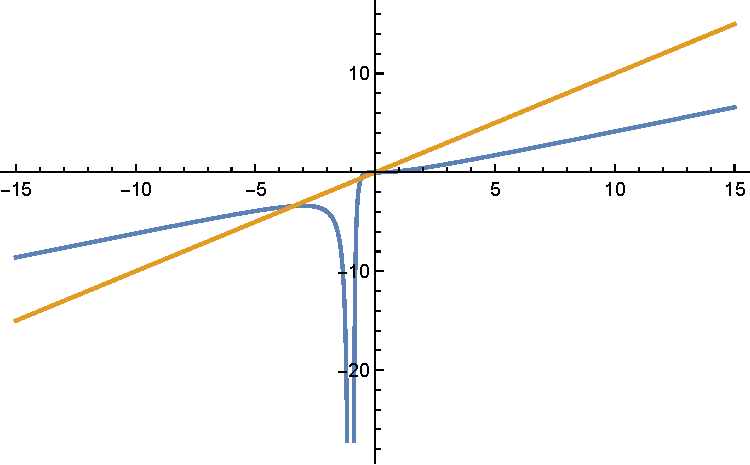
\includegraphics{Function1.pdf}
		\caption{$f(x) = \dfrac{x^3}{2(x + 1)^2}$}
	\end{figure}
\end{solution}

\begin{example}
	Analyse
	\begin{equation*}
	f(x) = 
	\begin{cases}
		e^{-\sfrac{1}{x^2}} &;\quad x \neq 0\\
		0 &;\quad x = 0
	\end{cases}
	\end{equation*}
\end{example}

\begin{solution}
	Domain of definition:
	\begin{align*}
		D(f) &= \mathbb{R}
	\end{align*}
	
	The graph intersects the axes only at $(0,0)$.\\
	
	The function is even and non-periodic.\\
	
	\begin{align*}
		f'(0) &= \lim\limits_{h \to 0} \dfrac{f(h) - f(0)}{h}\\
		&= 0
		x > 0 \implies f'(x) > 0\\
		x < 0 \implies f'(x) < 0
	\end{align*}
	Therefore, $f$ is monotonically decreasing in $(-\infty, 0)$ and monotonically increasing in $(0, \infty)$.\\
	
	$f$ is convex downwards in $\left( -\sqrt{\dfrac{2}{3}}, \sqrt{\dfrac{2}{3}} \right)$ and convex upwards in $\left( -\infty, -\sqrt{\dfrac{2}{3}} \right) \cup \left( \sqrt{\dfrac{2}{3}}, \infty \right)$.\\
	
	$y = 1$ is a horizontal asymptote.
	
	\begin{figure}[h]
		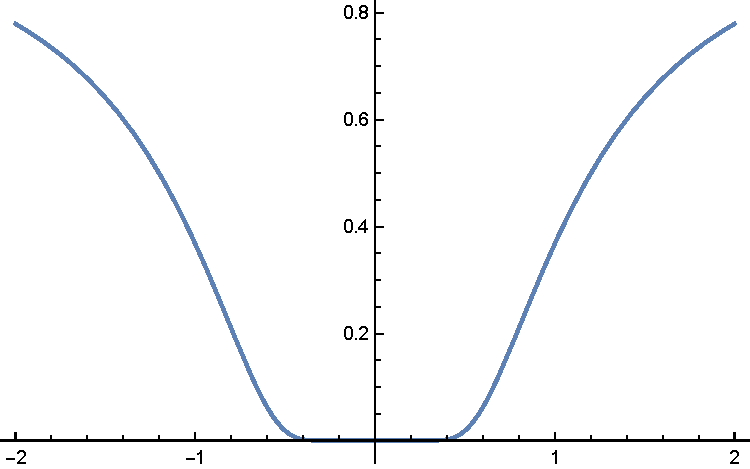
\includegraphics{Function2.pdf}
	\end{figure}
\end{solution}

\end{document}

